\chapter{硬件系统、软件算法架构设计与系统信息流向}
\section{引言}
上述3、4章节具体阐述了导航系统的两个层级之间的关系、区别以及具体设计方案。
但是导航系统的工程实现还需要在方案设计的基础之上进行硬件平台的搭建与软件
架构的设计。本章重点介绍根据上述两章的设计方案进行的硬件选型与相应的软件
架构设计,并且给出系统中信息的流动方向,并且在实地测验中总结当前系统的实
用优点与不足,为后续对系统的改进与园区内实用功能增添指明方向。

\section{硬件系统设计}
硬件系统主要分为两个方面来讲述,分别是硬件的选型与硬件的搭建方案。首先是
硬件的选型首要依据是其与实验室底盘平台的适配性,其次是其成本。而硬件的
搭建主要是根据当前所具备的硬件条件,如何有效规划这些硬件的使用与配合,保
障系统在有限的硬件条件下,发挥出最佳的效果。
小车的整体外形设计如下所示,展示小车的斜视与侧视图。
\begin{figure}[ht]
    \centering
    \includegraphics[scale=0.5]{robotModel1.png}
    \caption{移动机器人实物图}
\end{figure}

\subsection{硬件选型}
在移动机器人的硬件组成中,小零件相当多且繁杂,但是有几类硬件的重要性对于系
统性能甚至于功能来说,至关重要。他们分别是执行计算的中央处理单元——计算平台;
驱动执行部件——机器人底盘;环境感知传感器——激光雷达;高精度车载组合定位模块
——RTK。
首先最重要的计算单元我们根据系统算法的要求,且根据目前实验室对算法的更新频
率以及更新便捷性,选择了搭载了算力强大的CPU与GPU的Legion型号大算力计算机。
校园环境下的使用证明,选型正确且留有了相当充足的计算裕量。

\subsubsection{智能无人平台计算核心LENOVO LEGION笔记本}
计算核心是整个系统的重中之重,相当于是人类的大脑,承担一切的计算工作,并且
处理相应的输入信息,最终将处理得到的结果转化为控制指令,完成对车辆的控制。
其性能参数为

\textcolor{red}{此处插入表格}

导航系统运行的计算机操作系统为Ubuntu 18.04,具体通信平台为ROS-Melodic-deskfull。
以下是计算核心的实物图。
\begin{figure}[ht]
    \centering
    \includegraphics[scale=0.5]{computer.jpg}
    \caption{计算核心实物图}
\end{figure}


\subsubsection{煜禾森FR07阿克曼线控底盘}
FR-07 是一款全能型机器人线控移动平台,它采用和汽车类似的结构—阿克曼结构,
驱动后置,相对于差动结构的底盘,在普通路面上 FR-07 具有更快速的行走能力
和较强的负载能力,同时对轮胎的磨损也更小,搭配整体桥式悬挂,能够通过减速
带等常见障碍物,更适合长时间室外运行;并且,该底盘是基于车规级 VCU 构建
的自动驾驶底层,采用CAN 总 线管理,具有高精度、车规级、模块化等特点;通
过搭载激光雷达、GPS、机械臂等上部模 块和导航系统广泛应用于自动驾驶、无人巡
检、物流、运输配送、科研以及各种新的需要移动底盘的应用探索中。
线控底盘通过CAN盒与计算核心相连,接口类型为USB,通信的数据类型为yhs\_can\_msgs。
具体控制方式是,计算核心输出geometry\_msgs::TwistStamped类型消息,此消息会
在相应的fr07\_cntrol被转化成yhs\_can\_msgs类型消息,从而达到计算核心和底盘的
通信。我们的底盘自带48V/20AH的锂电池,可向车体持续供电5h以上,并且此电源可
向外用设备,如激光雷达、RTK等供电,供电标准为5A-12V/15A-5V/4A。且在此基础
上配备有可移动的220V稳压电源,用于户外向计算核心单独供电,保障整体用电安全性。

其通信相关的参数为:

\textcolor{red}{此处插入表格}

关于其他使用的性能参数为:

\textcolor{red}{此处插入表格}

下图是它的实物图。
\begin{figure}[ht]
    \centering
    \includegraphics[scale=0.3]{chassis.jpg}
    \caption{底盘实物图(无雷达支架)}
\end{figure}

\subsubsection{Velodyne VLP-16激光雷达}
不可否认目前已经出现了十分优秀的国产激光雷达产品以及厂商,例如禾赛科技、
速腾聚创等。但是由于实验室平台搭建开始于2-3年前,当时条件下,Velodyne
的VLP-16型号激光雷达是十分适配实验室的移动智能机器人的,并且十分符合团队
对园区场景下机器人“性能可观、成本可控”的设计理念。

此款雷达的性能参数为:

\textcolor{red}{此处插入表格}
性能参数:测量距离100、重量830g、360°水平视场扫描、±15°的垂直视场、竖直分辨率2°、水平分辨率在实验室小车上10Hz下为0.2°
使用方法:智能无人平台计算平台为LENVOV LEGION笔记本,系统Ubuntu18.04, ROS版本:Melodic.

\textcolor{red}{可以加入对雷达坐标系、点的存储等问题的分析描述}

实物图如下:
下图是它的实物图。

\begin{figure}[ht]
    \centering
    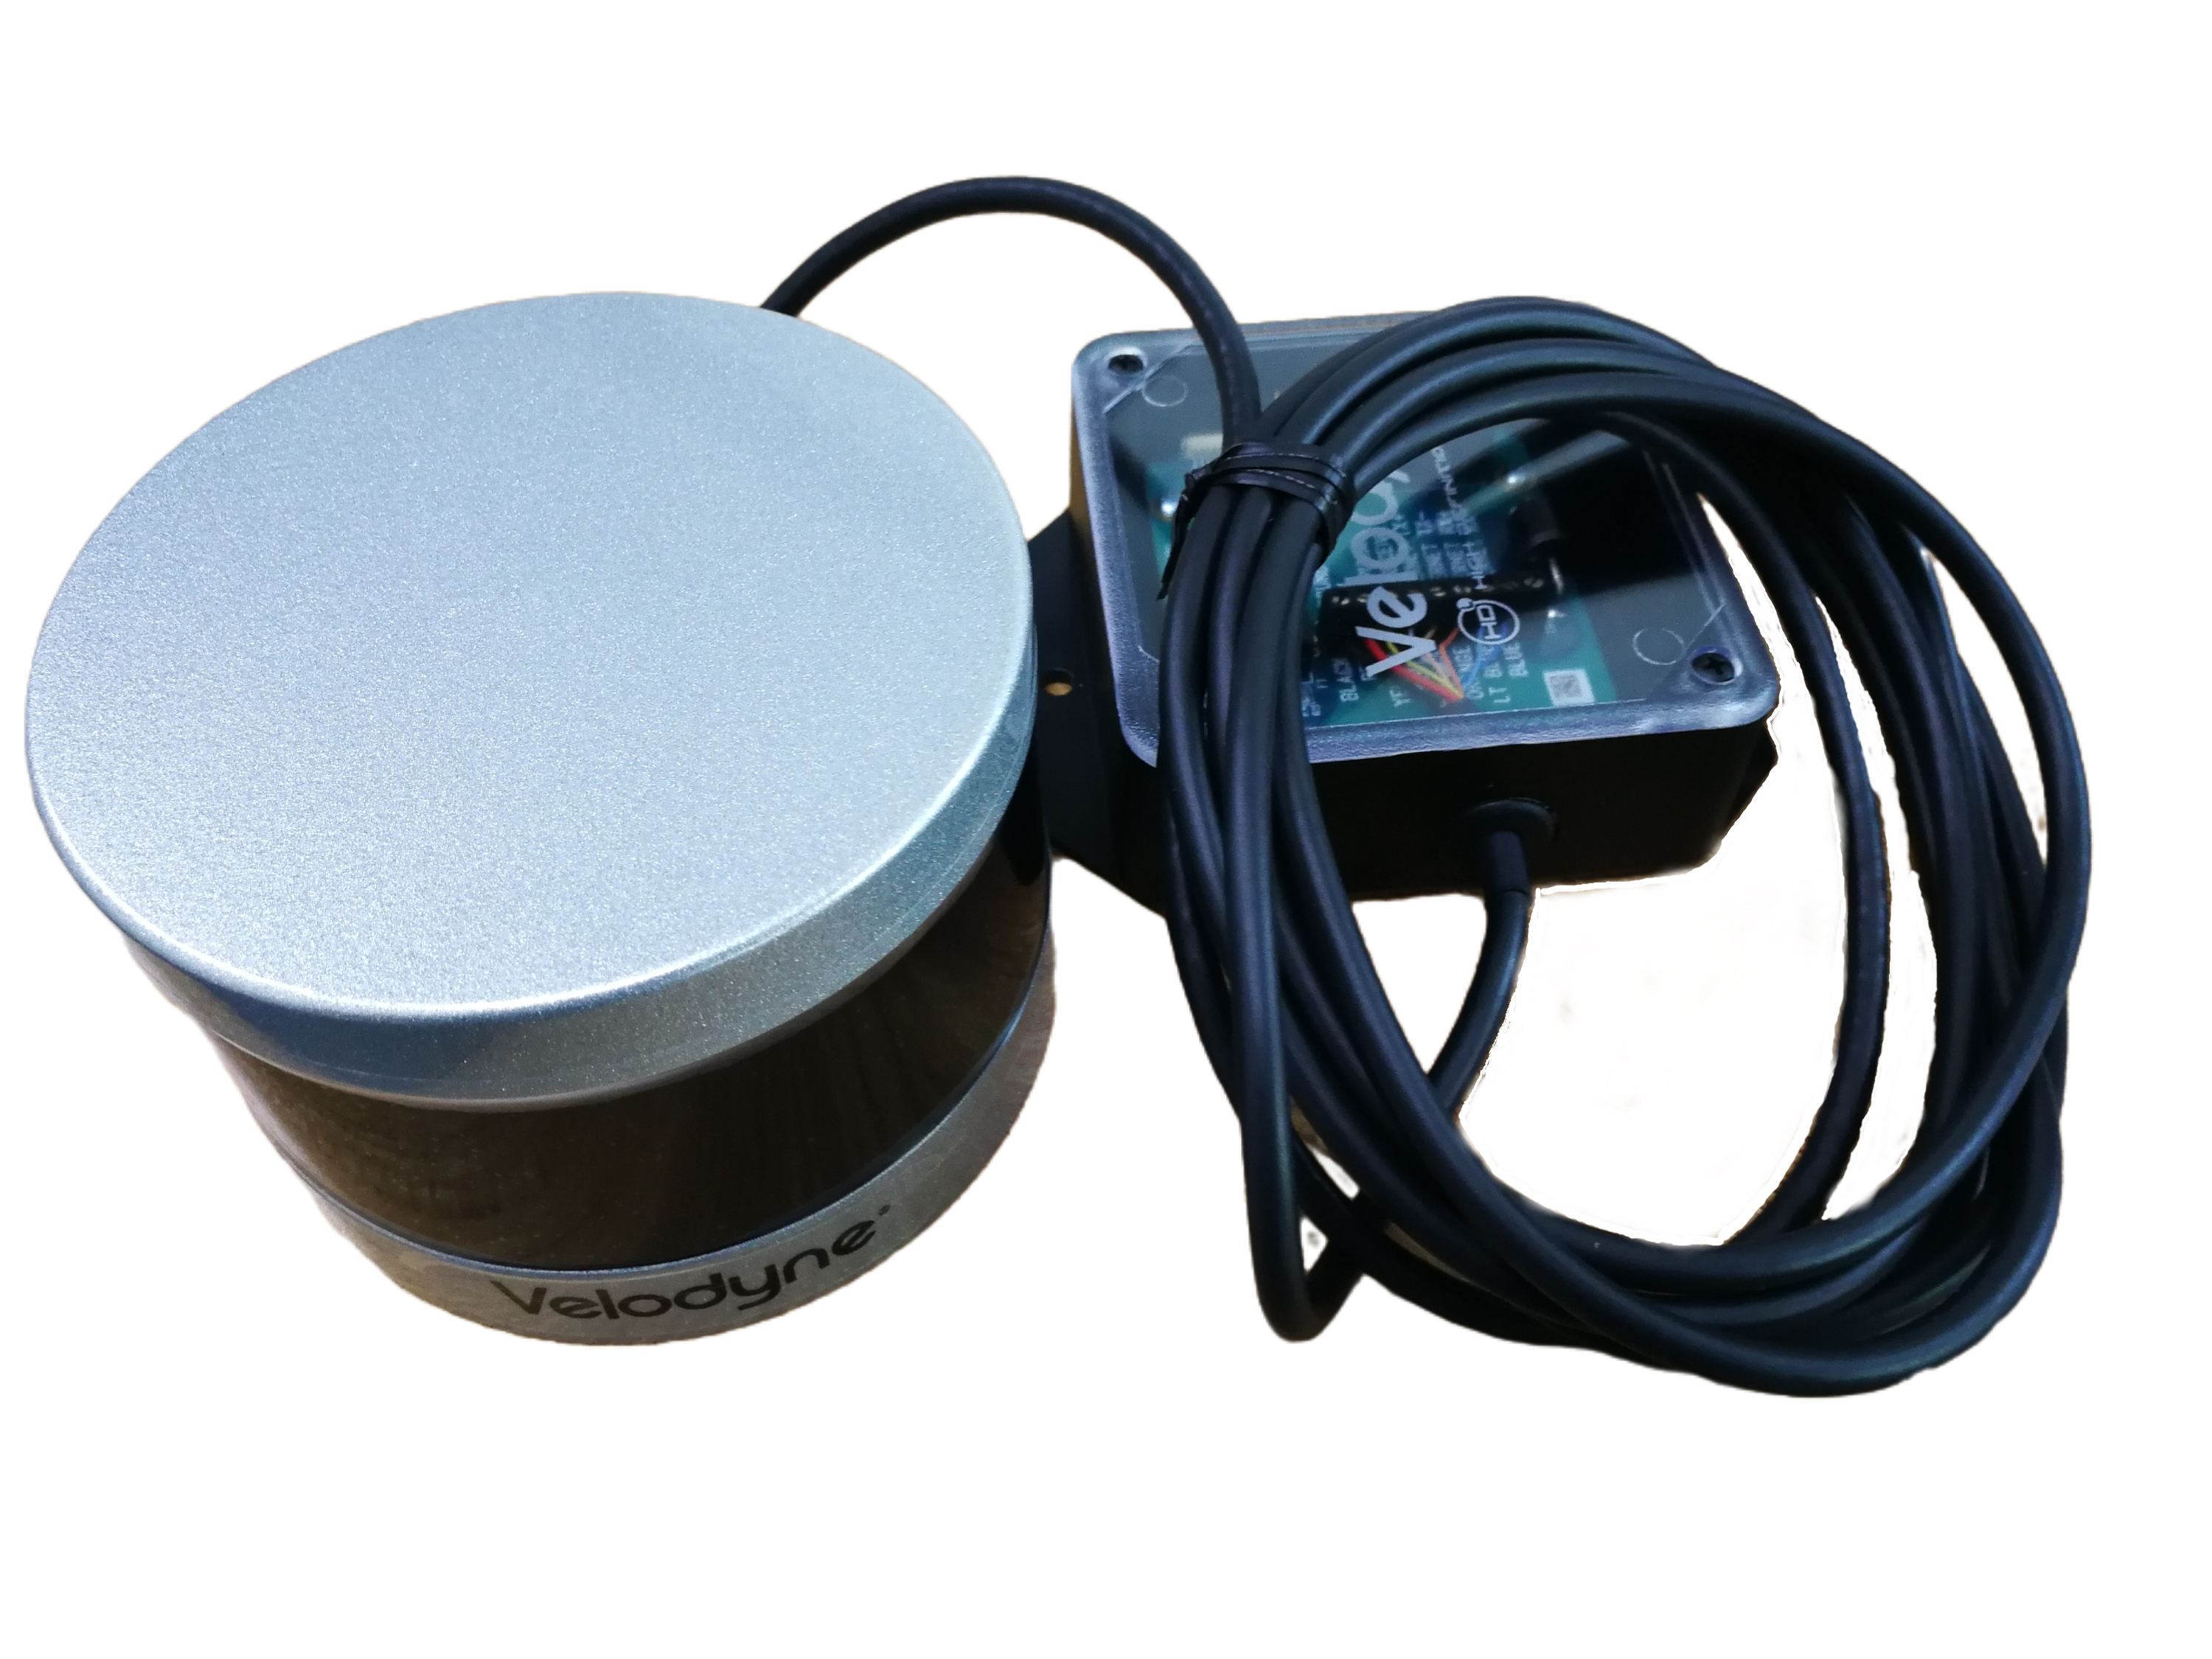
\includegraphics[scale=0.112]{3lidar.png}
    \caption{VLP-16实物图}
\end{figure}

\subsubsection{Ydlidar TG 30激光雷达}
底盘上安装3D激光雷达的位置决定了其对低矮且靠近移动机器人位置的物体
扫描能力相当局限。而在系统移动过程中,充分考虑了园区场景内的特点,
例如低矮的石凳、快速移动的小猫咪和流浪狗,在移动过程中针对此类低矮
物体的避障,可以通过2D激光雷达补盲的方式。

2D激光雷达的性能参数如下:

\textcolor{red}{此处插入表格}

2D激光雷达的配置与实物图如下所示:

\begin{figure}[ht]
    \centering
    \includegraphics[scale=0.5]{2dlidar.png}
    \caption{2D激光雷达安装实物图}
\end{figure}
安装后,对2D激光雷达和3D激光雷达进行标定,并将不同坐标系下的点云整合到同一坐标系下,整合后的点云如图所示:
\begin{figure}[ht]
    \centering
    \includegraphics[scale=0.5]{3d_2dpoints.png}
    \caption{点云叠加图及其tf关系}
\end{figure}
图中亦展示了车后轮中心base\_link与两个传感器坐标系之间的欧式变换关系。

当3D激光雷达与2D激光雷达组合后,系统的视野范围扩展到了车前方的低矮视野盲区,对低矮物体的扫描结果如下图所示:
\begin{figure}[ht]
    \centering
    \includegraphics[scale=0.4]{multiAndone.png}
    \caption{不同数量的低矮障碍物扫描视野情况图}
\end{figure}
图中白色部分为2D激光雷达扫描点,彩色部分为3D激光雷达扫描点 由图中的上两图可以看出,远处的低矮物体(蓝框),既有3D激光雷达的扫描点亦有2D激光雷达的扫描点,近处(黄框)的高处人身体有两者的扫描点,而低矮圆凳仅有2D激光雷达扫描线,同时系统已经做出反应,对车体前方的路径做出了筛选。下三图更加佐证了这一功能,近处垃圾桶位置无彩色扫描点,仅有2D激光雷达的白色扫描线,并且相应的路径已有筛选。证明系统已经具备低矮盲区的扫描能力,不在对车身周围的低矮物体会有意外碰撞。

\subsubsection{车载组合高精度定位模块}
定位是导航系统中尤为重要的一个模块,在具备了全局的先验地图之后,想要
根据全局地图进行全局的路径规划,需要确定自身的实际位置。在依托于全局
地图的导航中,我们通过车载组合高精度定位模块进行自身的实际定位。
硬件的选型为中海达Hi-Target RTK iNAV2型号。其定位的性能参数为

\textcolor{red}{此处插入表格}

RTK实物图如图所示:
\begin{figure}[ht]
    \centering
    \includegraphics[scale=0.5]{RTK.png}
    \caption{RTK实物三视图}
\end{figure}

其中上述展示的为其主体,在使用过程中,RTK包括了两个GPS信息接收终端,
分别安装在移动机器人的前后位置,用以接收、校正GPS卫星定位数据。



\subsection{硬件连接与信息交互}
上述介绍了对硬件的选型,确定选型之后,便是考虑如何对硬件进行连接。

为了关系的清晰性与明确性,连接图的构建抛弃了所有的辅助链接设备,例如
CAN盒等,只展示最核心的几大部件的相互连接关系。如下图所示:

\begin{figure}[ht]
    \centering
    \includegraphics[scale=0.5]{hardwareConnect.png}
    \caption{系统硬件连接与硬件数据流向图}
\end{figure}

计算核心在硬件中扮演的角色类似于人体中的大脑,无论是外界输入的信号,还是
本身内部想要发出的执行指令都是通过计算核心在其中协调,并给出数据信号,完成
整个过程。
两个激光雷达类似于人类的眼睛,在整个导航系统中负责提取环境信息,并且将环境
信息以点云的形式交给计算核心进行处理,类似于通过点云数据理解环境的过程,而
计算核心又可以通过自身需求对采集点云的激光雷达发出一定要求,例如采集的频率;
RTK主要是通过卫星定位对移动机器人的当前位置进行更新,智慧生物可以自然地对
自身所处位置进行评估更新修正,但是移动机器人无法做到这一点,所以RTK以计算
核心下达的更新指令为依据,以需求频率对移动机器人的位置进行更新反馈,并在此
过程中,将定位信息反馈给计算核心,再由计算核心调动参与移动机器人的其他功能;
在得到了环境信息以及自身在环境中的所处位置之后,经过一系列的导航算法处理,移
动机器人会根据导航系统的安排,执行具体的动作到达相应位置,在这个过程中,主要
是依靠底盘作为命令的执行器件,计算核心将控制命令发送给CAN总线,总线再将命令
解读成阿克曼底盘可以理解的数字指令,交付执行。

如上流程便是各个主要器件参与导航系统的功能角色,接下来本文会在此基础上,结合
第3、4章的导航系统设计部分,完成呈现整个导航系统的流程框图。

\section{导航系统的实现及其信息流向}

整个多层级导航系统的大致信息流向是高层导航规划出一系列路径点,底层导航根据
环境信息以及自身定位,完成碰撞避免,安全执行一个个路径点的到达任务,当到达最
后一个目标点时,整个导航任务完成。宏观上来看,多层级导航系统分为两个子系统,
分别是高层系统和底层导航,两者之间通过局部路径点作为信息沟通的桥梁。宏观的
框图如下:

\begin{figure}[ht]
    \centering
    \includegraphics[scale=0.5]{navi_info1.png}
    \caption{高层导航与底层导航信息流向图}
\end{figure}

在此整体的架构图基础之上,分别展开对底层导航和高层导航的架构图详细介绍。
在宏观的系统架构之上,底层导航和高层导航之间除了少量关联之外,多数情况下
功能是分别处理各自输入信息,因为对两个子系统做更加深入的了解。

\section{底层导航的架构与信息流程}
对于移动机器人的多层级导航系统而言,第一步是构建其底层导航系统,原因在于
底层负责最基本的驱动执行与避障。无论何种形式的移动机器人,都需要从这个基础
功能出发。

在第3章节中介绍了底层导航系统的设计思路与相应的算法原理,本节则是侧重于对
思路的实现与具体运行过程中的相关信息解读。

\begin{figure}[ht]
    \centering
    \includegraphics[scale=0.5]{localnavi-processing.png}
    \caption{底层导航处理流程图}
\end{figure}

